{最短路径问题是图论研究中的一个经典算法问题,{旨在寻找图(由结点和路径组成的)中两结点之间的最短路径}。算法具体的形式包括:}

{{第一种:}{迪杰斯特拉算法}{,}此算法是一种}{确定起点求最短路径的问题。}

{{{第二种:}{弗洛伊德算法}{,}此算法是求图中任意一对顶点间的最短路径。}}

{\textbf{1. 迪杰斯特拉算法}}

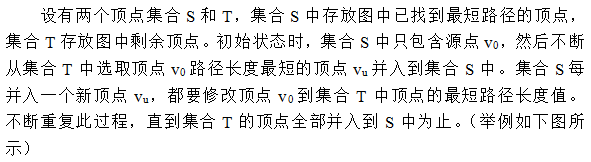
\includegraphics[width=3.70833in,height=1.02083in]{png-jpeg-pics/F5BB29135CB5BF3A38D4436EC07F7F87.png}

{}

{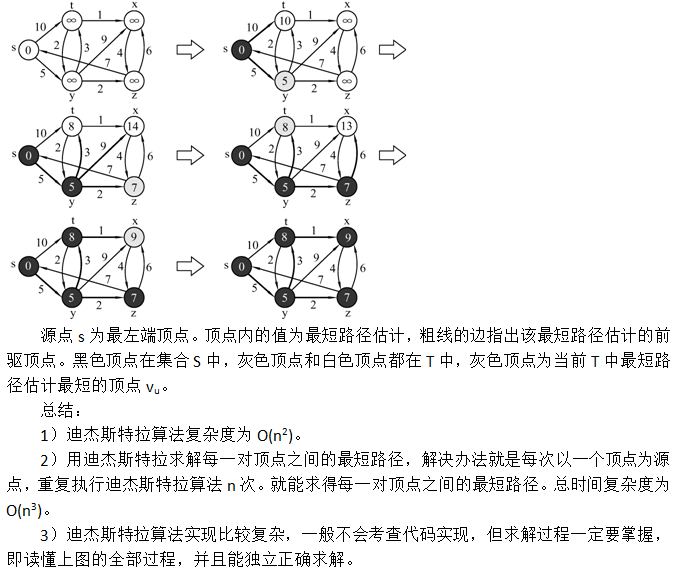
\includegraphics[width=3.70833in,height=3.14583in]{png-jpeg-pics/5A3D0661340FA3AE873B2E5D0908E9F7.png}\\
}

{\textbf{2. 弗洛伊德算法(可选看,掌握\textbf{迪杰斯特拉算法}即可)}}

{\textbf{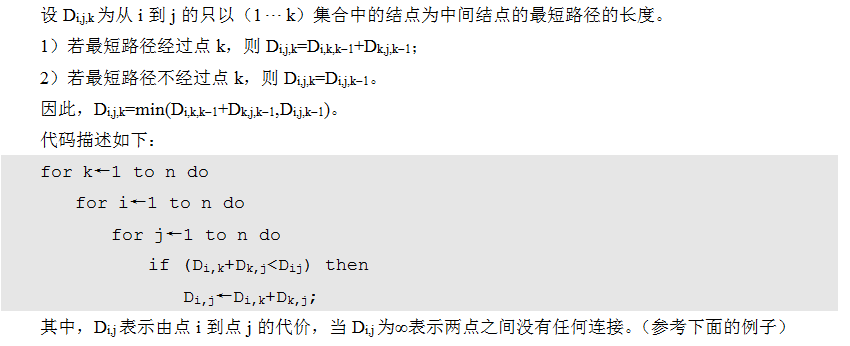
\includegraphics[width=3.70833in,height=1.51042in]{png-jpeg-pics/100728F2DD647E5541BAE5A9650BCE86.png}\\
}}

{\textbf{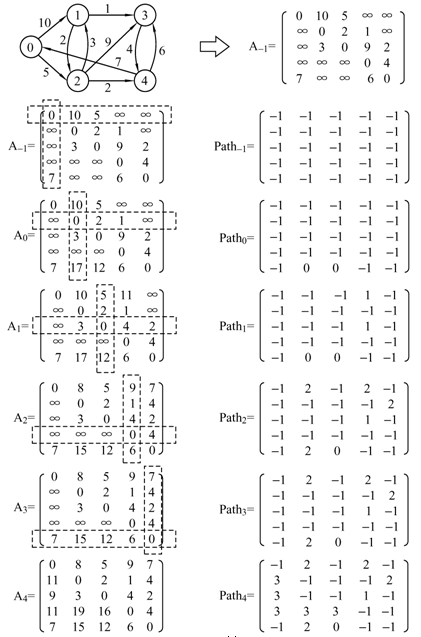
\includegraphics[width=3.70833in,height=5.61458in]{png-jpeg-pics/FCB984767E7C573FB82B60E31CC8018E.png}\\
}}

{\textbf{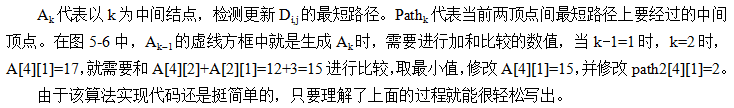
\includegraphics[width=3.70833in,height=0.54167in]{png-jpeg-pics/7B265A48E834B4FFEE752E6EDF63F26C.png}\\
}}

{\textbf{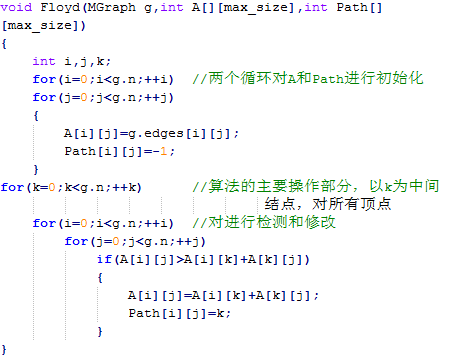
\includegraphics[width=3.70833in,height=2.94792in]{png-jpeg-pics/E05C0079C0652F8DAB296970044FA836.png}\\
}}
